% Diese Datei ist Teil des Buchs "Schreibe Dein Programm!"
% Das Buch ist lizensiert unter der Creative-Commons-Lizenz
% "Namensnennung - Weitergabe unter gleichen Bedingungen 4.0 International (CC BY-SA 4.0)"
% https://creativecommons.org/licenses/by-sa/4.0/deed.de

\chapter{Videospiele programmieren}
\label{cha:representation-and-state}

In diesem Kapitel programmieren wir zum ersten Mal ein vollständiges,
benutzbares Programm, nämlich ein kleines Videospiel.  Dafür brauchen
wir zwei Zusätze für die Lehrsprache in DrRacket, die Teachpacks
\texttt{image.rkt} und \texttt{universe.rkt}.  Ersteres ist für das
Anzeigen der Grafik zuständig (wir haben es im ersten Kapitel schon
einmal benutzt), und \texttt{universe.rkt} ist dafür da, die Grafiken
zu bewegen und interaktiv zu machen.

\section{Bilder mit \texttt{image.rkt}}

Für die Grafikprogrammierung mit \drscheme{} laden wir ein sogenanntes
\textit{Teachpack\index{Teachpack}}, ein kleiner Sprachzusatz, in
diesem Fall mit einer Reihe von Funktionen zur Erzeugung von Bildern.
Wir sind ihm bereits in Abschnitt~\ref{sec:rechnen-mit-bildern} auf
Seite~\pageref{sec:rechnen-mit-bildern} begegnet: Um das Teachpack zu
laden, musst Du im Menü \texttt{Sprache} (oder \texttt{Language} in
der englischen Ausgabe) den Punkt \texttt{Teachpack hinzufügen}
(\texttt{Add teachpack}) anwählen, und im dann erscheinenden
Auswahl-Dialog die Datei
\texttt{image.rkt\index{image.rkt@\texttt{image.rkt}}} auswählen.

Dieses Kapitel beschreibt die wichtigsten Funktionen des Teachpacks,
aber es gibt noch viel mehr davon.  Du kannst Dokumentation dazu
finden, indem Du in DrRacket im \texttt{Hilfe}- oder \texttt{Help}-Menü
auf die Racket-Dokumentation klickst, und dort nach
\texttt{2htdp/image} im Suchfeld eintippst.\footnote{Zum Zeitpunkt der
  Drucklegung leider nur auf Englisch.  Wir arbeiten an einer
  deutschen Übersetzung.}

\subsection{Einfache Bilder}

Im Teachpack \texttt{image.rkt} erzeugen verschiedene Funktionen
einfache Bilder.  So hat zum Beispiel die Funktion \texttt{rectangle}
folgende Signatur:\index{rectangle@\texttt{rectangle}}
% 
\begin{lstlisting}
(: rectangle (real real mode color -> image))
\end{lstlisting}
%
Dabei sind die ersten beiden Argumente Breite und Höhe eines Rechtecks
in Pixeln.
Das Argument mit Signatur \lstinline{mode}\index{mode@\texttt{mode}} ist eine Zeichenkette, die
entweder \lstinline{"solid"} oder \lstinline{"outline"} sein muss. Sie bestimmt,
ob das Rechteck als durchgängiger Klotz oder nur als Umriss gezeichnet
wird.  Das Argument mit der Signatur \lstinline{color}\index{color@\texttt{color}} ist eine
Zeichenkette, die eine Farbe (auf Englisch) bezeichnet, 
zum Beispiel \lstinline{"red"}, \lstinline{"blue"}, \lstinline{"yellow"},
\lstinline{"black"}, \lstinline{"white"} oder \lstinline{"gray"}.  Als Ergebnis
liefert \lstinline{rectangle} ein Bild, das von der \drscheme{}-REPL
entsprechend angezeigt wird wie andere Werte auch.  Beispiel:
%
\begin{lstlisting}
(rectangle 100 30 "outline" "brown")
|\evalsto| |
\includegraphics[scale=0.5]{i1world/rectangle}|
\end{lstlisting}
%
Als Farbe geht übrigens auch \lstinline{"transparent"}, die das Bild
durchsichtig beziehungsweise unsichtbar macht.  (Wozu ist ein
unsichtbares Bild gut, fragst Du vielleicht. Zum Beispiel, wenn wir
ein kleineres Bild nicht ganz mittig platzieren wollen~-- dann können
es auf ein transparentes Bild legen.)

Es gibt es noch weitere Funktionen, die 
geometrische Figuren zeichnen:\index{circle@\texttt{circle}}
%
\begin{lstlisting}
(: circle (real mode color -> image))
\end{lstlisting}
%
Die \lstinline{circle}-Funktion liefert einen Kreis, wobei das erste
Argument den Radius angibt.  Die \lstinline{mode}- und
\lstinline{color}-Argumente sind wie bei \lstinline{rectangle}.
Beispiel:
%
\begin{lstlisting}
(circle 50 "solid" "red")
|\evalsto| |
\includegraphics[scale=0.5]{i1world/circle}|
\end{lstlisting}
%
\begin{lstlisting}
(: ellipse (real real mode color -> image))
\end{lstlisting}
%
\index{ellipse@\texttt{ellipse}}Diese Funktion liefert eine Ellipse,
wobei das erste Argument die Breite und das zweite die Höhe angibt.
Beispiel:
%
\begin{lstlisting}
(ellipse 50 100 "solid" "green")
|\evalsto| |
\includegraphics[scale=0.5]{i1world/ellipse}|
\end{lstlisting}
%
\begin{lstlisting}
(: triangle (real mode color -> image))
\end{lstlisting}
%
\index{triangle@\texttt{triangle}}Diese Funktion liefert ein nach oben
zeigendes gleichseitiges Dreieck, wobei das erste Argument die
Seitenlänge angibt.  Beispiel:
%
\begin{lstlisting}
(triangle 50 "solid" "gold")
|\evalsto| |
\includegraphics[scale=0.5]{i1world/triangle}|
\end{lstlisting}
%
\begin{lstlisting}
(: line (real real color -> image))
\end{lstlisting}
%
\index{line@\texttt{line}}zeichnet eine Linie.  Der Aufruf
\lstinline{(line $w$ $h$ $c$)} liefert ein Bild
mit Breite $w$ und Höhe $h$, in dem die Linie von der linken oberen in
die rechte untere Ecke verläuft.  Falls die Linie entlang der anderen
Diagonale verlaufen soll, kannst Du einfach das Vorzeichen von $w$
oder von $h$ umdrehen.  Beispiele:
%
\begin{lstlisting}
(line 150 100 "blue")
|\evalsto| |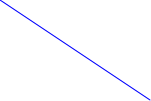
\includegraphics[scale=0.5]{i1world/line1}|
(line -150 100 "blue")
|\evalsto| |
\includegraphics[scale=0.5]{i1world/line2}|
\end{lstlisting}
%
Wir können auch ein Bild erzeugen, in dem Text steht, und zwar mit der
Funktion \lstinline{text}\index{text@\texttt{text}}, die folgende Signatur hat:
%
\begin{lstlisting}
(: text (string real color -> image))
\end{lstlisting}
%
Die Zahl ist die Höhe der Buchstaben.  Beispiel:
%
\begin{lstlisting}
(text "Schreibe Dein Programm!" 20 "red")
|\evalsto| |
\includegraphics[scale=0.5]{i1world/text}|
\end{lstlisting}
%
Manchmal reichen einfache Rechtecke und Kreise nicht aus und wir
wollen komplexere Formen erzeugen.  Eine Möglichkeit ist die Funktion
\lstinline{polygon}\index{polygon@\texttt{polygon}}, die ein n-Eck
zeichnet.  Sie hat folgende Signatur:
%
\begin{lstlisting}
(: polygon ((list-of (mixed posn pulled-point)) mode color -> image)) 
\end{lstlisting}
%
Diese Funktion akzeptiert eine Liste von Eckpunkten und die üblichen
\lstinline{mode}- und \lstinline{color}-Argumente.  Ein Eckpunkt 
muss entweder zur Signatur \lstinline{posn} oder zu
\lstinline{pulled-point} gehören.  Das sind eingebaute Record-Typen,
bei denen \lstinline{posn}\index{posn@\texttt{posn}} so definiert sein könnte:
%
\begin{lstlisting}
(define-record posn
  make-posn
  posn?
  (posn-x real)
  (posn-y real))
\end{lstlisting}
%
Dieser Typ definiert also ganz normale kartesische Koordinaten mit X-
und Y-Komponente.  Hier ist ein Beispiel für ein Polygon mit solchen
Eckpunkten:
%
\begin{lstlisting}
(polygon (list (make-posn 0 0)
               (make-posn -20 40)
               (make-posn 120 0)
               (make-posn -20 -40))
         "solid"
         "plum")
|\evalsto| |
\includegraphics[scale=0.5]{i1world/polygon1}|
\end{lstlisting}
%
Bei \lstinline{posn}-Eckpunkten sind die Kanten also alles gerade
Linien.  Mit \lstinline{pulled-point}-Eckpunkten ist es möglich, die
Kanten zu Kurven zu machen.  Auch \lstinline{pulled-point} ist ein
Record-Typ, der so definiert sein könnte:
%
\begin{lstlisting}
(define-record pulled-point
 make-pulled-point
 pulled-point?
 (pulled-point-lpull real)
 (pulled-point-langle real)
 (pulled-point-x real)
 (pulled-point-y real)
 (pulled-point-rpull real)
 (pulled-point-rangle real))
\end{lstlisting}
%
Wie \lstinline{posn} hat auch \lstinline{pulled-point} eine X- und
eine Y-Koordinate.  Außerdem gibt es zwei "<Pull">- und zwei
"<Angle">-Komponenten, die spezifizieren, wie die Kanten gebogen
werden.  Abbildung~\ref{fig:pulled-point} zeigt, wie das
funktioniert:  Für jeden Eckpunkt gibt es eine Kante vom
vorigen Punkt~-- die \emph{eingehende} Kante~-- und die Kante zum nächsten
Punkt~-- die \emph{ausgehende} Kante.

\begin{figure}[tb]
  \centering
  \def\svgwidth{0.4\textwidth}
  \input{i1world/pulled-point.pdf_tex}
  \caption{Funktionsweise von \lstinline{pulled-point}}
  \label{fig:pulled-point}
\end{figure}
%
Die \lstinline{pulled-point-langle}-Komponente gibt den Winkel an, mit
dem die eingehende Kante gebogen wird, die
\lstinline{pulled-point-rangle}-Komponente den Winkel ist für die
ausgehende Kante zuständig.  Abbildung~\ref{fig:pulled-point} zeigt,
wie \lstinline{langle} und \lstinline{rangle} auf den Punkt mit der
Nummer~2 wirken: Die eingehende Kante kommt von Punkt~1 her, die
ausgehende Kante geht zu Punkt~3.  Die Komponenten
\lstinline{pulled-point-lpull} und \lstinline{pulled-point-rpull}
geben wann, wieviel die Kanten verbogen werden~-- das sind
typischerweise Zahlen zwischen 0 und 1.
%
\begin{lstlisting}
(polygon (list (make-pulled-point 1/2 0 0 0 1/2 -20)
               (make-posn -20 40)
               (make-pulled-point 1/2 -20 120 0 1/2 20)
               (make-posn -20 -40))
         "solid"
         "plum")
|\evalsto| |
\includegraphics[scale=0.5]{i1world/polygon2}|
\end{lstlisting}
%
\begin{figure}[tb]
  \centering
  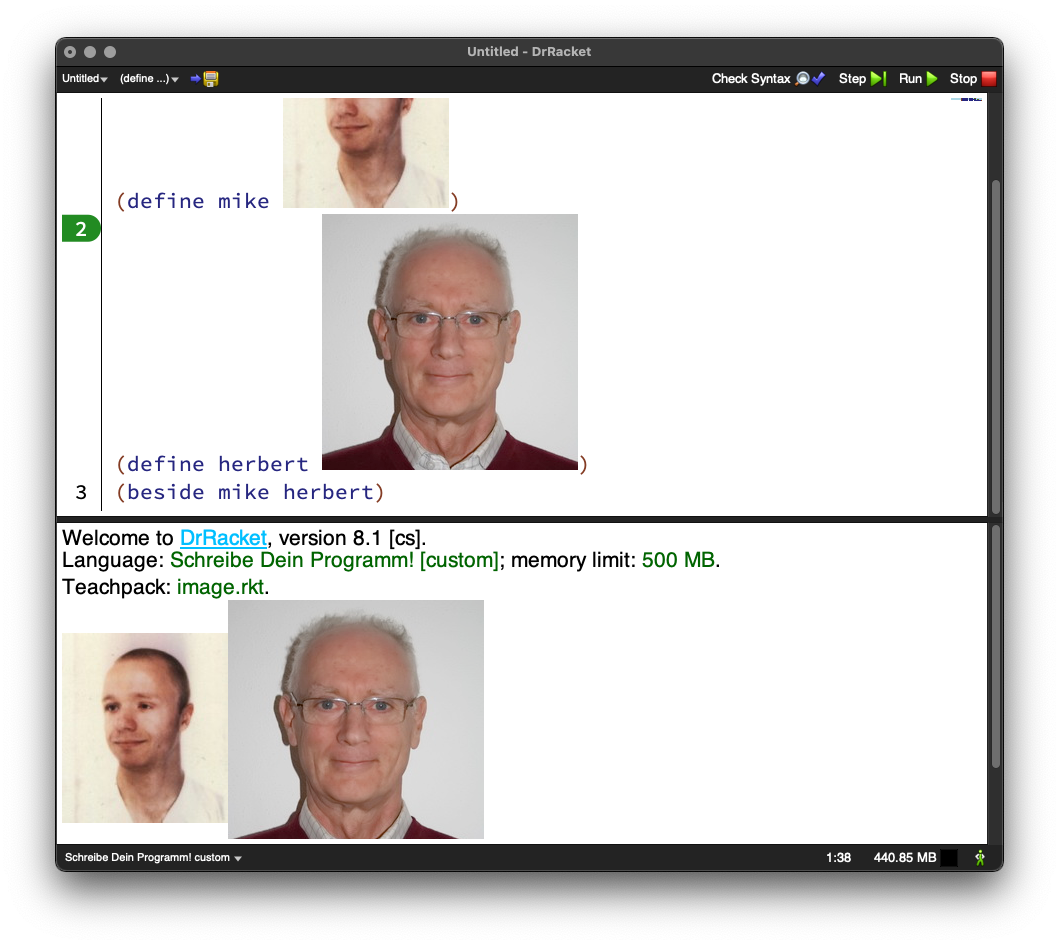
\includegraphics[height=0.4\textheight]{i1world/insert-image}
  \caption{Bilddatei in Programm einbetten}
  \label{fig:image-insert}
\end{figure}
Es ist auch möglich, externe Bilder-Dateien in
\texttt{image.rkt}-Bilder zu verwandeln.  Dazu dient der Menüpunkt
\texttt{Bild einfügen} im \texttt{Spezial}-Menü: \drscheme{} fragt
nach dem Namen einer Bilddatei, die dann in den Programmtext da
eingefügt wird, wo der Cursor steht.  Alternativ ist es möglich,
Bilder in anderen Applikationen auszuwählen und zu kopieren und dann
in DrRacket einzufügen.  Die eingefügten Bilder dienen dann als
Literale für Bild-Objekte.  Abbildung~\ref{fig:image-insert} zeigt ein
Beispiel.

Schließlich ermitteln die folgenden Funktionen Breite und Höhe
eines Bildes:\index{image-width@\texttt{image-width}}\index{image-height@\texttt{image-height}}
%
\begin{lstlisting}
(: image-width  (image -> natural))
(: image-height (image -> natural))
\end{lstlisting}
%

\subsection{Bilder zusammensetzen und verändern}

Da diese geometrischen Formen für sich genommen langweilig sind,
können wir mehrere Bilder zu einem zusammensetzen.

Zum Aufeinanderlegen gibt es die Funktion
\lstinline{overlay}\index{overlay@\texttt{overlay}}, die ein Bild
mittig auf ein anderes Bild drauflegt.  Das Bild, das bei
\lstinline{overlay} herauskommt, ist groß genug, dass beide
Eingabebilder genau hineinpassen.  Signatur:
%
\begin{lstlisting}
(: overlay (image image -> image))
\end{lstlisting}
%
Beispiel:
%
\begin{lstlisting}
(overlay
  (circle 50 "solid" "gold")
  (rectangle 100 100 "solid" "blue"))
|\evalsto| |
\includegraphics[scale=0.5]{i1world/overlay}|
\end{lstlisting}
%
Mittig ist nicht immer das richtige Arrangement für zwei Bilder, die
übereinandergelegt werden.  Die
Funktion~\lstinline{overlay/xy}\index{overlayxy@\texttt{overlay/xy}}
erlaubt, das untere Bild gegenüber dem oberen in X- und Y-Richtung zu
verschieben.  Hier ist die Signatur:
%
\begin{lstlisting}
(: overlay/xy (image real real image -> image))
\end{lstlisting}
%
Beispiel:
%
\begin{lstlisting}
(overlay/xy
  (circle 50 "solid" "gold")
  10 -20
  (rectangle 100 100 "solid" "blue"))
|\evalsto| |
\includegraphics[scale=0.5]{i1world/overlayxy}|
\end{lstlisting}
%
Das Beispiel zeigt, das auch \lstinline{overlay/xy} das Ergebnisbild
gerade so groß macht, dass die beiden Eingabebilder hineinpassen.

Manchmal macht auch \lstinline{overlay/xy} nicht das richtige, nämlich
wenn einfach nur ein Objekt in eine "<Szene"> platziert werden soll,
zum Beispiel das Gürteltier auf einem Straßenabschnitt.  In dem Fall
wollen wir genau wie bei \lstinline{overlay/xy} kontrollieren, an
welchen Koordinaten das daraufgelegte Bild erscheint, aber das Bild
soll nicht größer werden, wenn zum Beispiel ein Teil des Gürteltiers
über den Straßenabschnitt hinausragt.  Diese Aufgabe erledigt die
Funktion
\lstinline{place-iamge}\index{place-image@\texttt{place-image}}, deren
Signatur der von \lstinline{overlay/xy} entspricht:
%
\begin{lstlisting}
(: place-image (image real real image -> image))
\end{lstlisting}
%
Die beiden Koordinaten werden allerdings anders als bei
\lstinline{overlay/xy} nicht relativ zur mittigen Anordnung
interpretiert.  Stattdessen geben die beiden Koordinaten die Position
im zweiten Bild an, wo die Mitte des ersten Bilds platziert wird,
ausgehend von der oberen linken Ecke des ersten Bildes.  Beispiel:
%
\begin{lstlisting}
(place-image
  (circle 50 "solid" "gold")
  40 70
  (rectangle 100 100 "solid" "blue"))
|\evalsto| |
\includegraphics[scale=0.5]{i1world/place-image}|
\end{lstlisting}
%
Die Funktion \lstinline{place-image} hat noch eine große Schwester
\lstinline{place-image/align}.\index{place-image-align@\texttt{place-iamge/align}}\label{func:place-image-align}
Während \lstinline{place-image} den Bezugspunkt immer in der Mitte des
ersten Bilds setzt, erlaubt \lstinline{place-image} auch anderee
Bezugspunkte.  Hier die Signatur:
%
\begin{lstlisting}
(: place-image/align (image real real x-place y-place image -> image
\end{lstlisting}
%
Die Signaturen \lstinline{x-place} und \lstinline{y-place} könnten
folgendermaßen definiert sein:
%
\begin{lstlisting}
(define x-place (signature (enum "left" "right" "center")))
(define y-place (signature (enum "top" "bottom" "center")))
\end{lstlisting}
%
Diese Argumente geben also an, ob der Bezugspunkt horizontal am linken
oder rechten Rand oder in der Mitte liegt und vertikal oben, unten
oder in der Mitte:
%
\begin{lstlisting}
(place-image/align
  (circle 20 "solid" "gold")
  40 70 "left" "center"
  (rectangle 100 100 "solid" "blue"))
|\evalsto| |
\includegraphics[scale=0.5]{i1world/place-image-align1}|
(place-image/align
  (circle 20 "solid" "gold")
  40 70 "right" "center"
  (rectangle 100 100 "solid" "blue"))
|\evalsto| |
\includegraphics[scale=0.5]{i1world/place-image-align2}|
(place-image/align
  (circle 20 "solid" "gold")
  40 70 "center" "center"
  (rectangle 100 100 "solid" "blue"))
|\evalsto| |
\includegraphics[scale=0.5]{i1world/place-image-align3}|
(place-image/align
  (circle 20 "solid" "gold")
  40 70 "center" "top"
  (rectangle 100 100 "solid" "blue"))
|\evalsto| |
\includegraphics[scale=0.5]{i1world/place-image-align4}|
(place-image/align
  (circle 20 "solid" "gold")
  40 70 "center" "bottom"
  (rectangle 100 100 "solid" "blue"))
|\evalsto| |
\includegraphics[scale=0.5]{i1world/place-image-align5}|
\end{lstlisting}
%
Die folgenden Funktionen \lstinline{above} und \lstinline{beside}
kennst Du vielleicht noch aus dem ersten Kapitel auf
Seite~\pageref{function:beside-above}.  Sie setzten zwei Bilder
übereinander respektive nebeneinander:
% 
\begin{lstlisting}
(: above  (image image -> image))
(: beside (image image -> image))
\end{lstlisting}
%
Manchmal sieht ein Bild gut aus, ist aber zu klein oder zu groß
geraten.  Die Funktion \lstinline{scale} kann es größer oder kleiner
machen.  Signatur:
\begin{lstlisting}
(: scale (real image -> image))
\end{lstlisting}
%
Beispiel:
%
\begin{lstlisting}
(define c (circle 20 "solid" "green"))
(beside (scale 0.5 c)
        c
        (scale 1 c)
        (scale 1.5 c)
        (scale 2 c)
        (scale 3 c))
|\evalsto| |
\includegraphics[scale=0.5]{i1world/scale}|
\end{lstlisting}

\section{Modelle und Ansichten}

In unserem Videospiel geht es um Gürteltiere auf dem texanischen
Highway.  Vielleicht erinnerst Du Dich, wir sind ihnen schon in
Abschnitt~\ref{sec:armadillo} auf Seite~\pageref{sec:armadillo}
begegnet.  Zur Erinnerung, hier ist der relevante Code dazu:
%
\begin{lstlisting}
; Ein Gürteltier hat folgende Eigenschaften:
; - Gewicht (in g)
; - lebendig oder tot
(define-record dillo
  make-dillo
  dillo?
  (dillo-weight natural)
  (dillo-alive? boolean))

(: make-dillo (natural boolean -> dillo))
(: dillo-weight (dillo -> natural))
(: dillo-alive? (dillo -> boolean))

(define dillo1 (make-dillo 55000 #t)) ; 55 kg, lebendig 
(define dillo2 (make-dillo 58000 #f)) ; 58 kg, tot
(define dillo3 (make-dillo 60000 #t)) ; 60 kg, lebendig
(define dillo4 (make-dillo 63000 #f)) ; 63 kg, tot

; Gürteltier überfahren
(: run-over-dillo (dillo -> dillo))

(define run-over-dillo
  (lambda (dillo)
    (make-dillo (dillo-weight dillo)
                #f)))
\end{lstlisting}
%
Die Datendefinition mit dem zugehörigen Code hält zwar einige Eigenschaften
von Gürteltieren fest, für ein Videospiel fehlt aber noch eine
grafische Darstellung.  Ebenso definiert \lstinline{run-over-dillo}
eine Operation auf Gürteltier-Objekten fest, aber auch die sagt nichts
zu einer grafischen Darstellung.  Eine solche Repräsentation mit
zugehörigen Operationen heißt in der Softwararchitektur auch
\textit{Modell}\index{Modell} oder auch
\textit{Domänenlogik}\index{Modell}, und bei größeren Softwaresystemen
ist es eine gute Idee, das Modell von der grafischen Darstellung zu
trennen, damit das Modell stabil bleiben kann, auch wenn die grafische
Darstellung geändert wird.

Die grafische Darstellung eines Modells nennen wir dessen
\textit{Ansicht}\index{Ansicht} (auf englisch
\textit{View}\index{View}).  Wenn wir uns also mit Gürteltieren als
Modell für ein Videospiel beschäftigen, müssen wir daraus eine Ansicht
in Form eines Bildes berechnen.

Wir warnen Dich schonmal vor: Der grafische Gestaltung in diesem
Kapitel fehlt es vorsichtig gesagt an Finesse.  Wir hoffen, Du kannst
es besser machen!

Um also aus einem \lstinline{dillo}-Wert ein Bild zu machen, werden
wir solch eine Funktion benötigen:
%
\begin{lstlisting}
; Gürteltier-Bild erzeugen
(: dillo-image (dillo -> image))
\end{lstlisting}
%
\begin{figure}[tb]
  \centering
  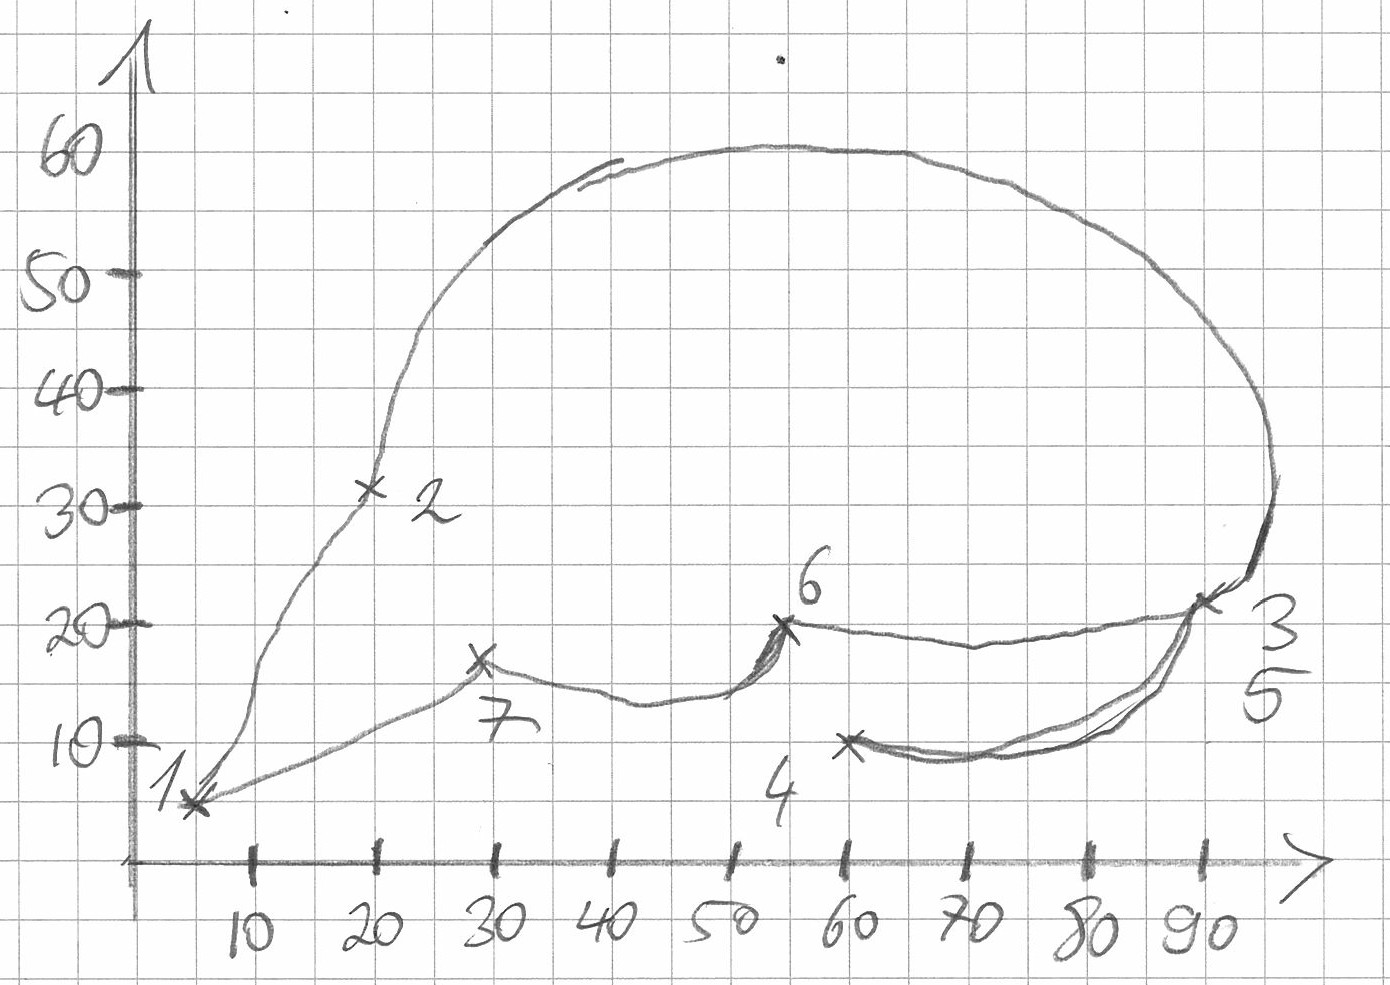
\includegraphics[width=0.6\textwidth]{i1world/dillo}
  \caption{Umriss eines Gürteltiers}
  \label{fig:dillo-body}
\end{figure}
Als Basis dafür machen wir erstmal ein Bild mit dem Körper des
Gürteltiers.  Zu diesem Zweck haben wir zunächst von Hand eine
Zeichnung mit dem Umriss des Gürteltiers in ein Koordinatensystem
gezeichnet und die Punkte markiert, an denen sich die Richtung des
Strichs abrupt ändert~-- also quasi die Ecken.  Diese Ecken haben wir
durchnummeriert und daraus haben wir dieses Polygon gemacht:
%
\begin{lstlisting}
(define dillo-body
  (overlay/xy (polygon
               (list (make-pulled-point
                      0.3 30
                      5 (- 60 5)
                      0.2 5)
                     (make-pulled-point
                      0.4 20
                      20 (- 60 32)
                      0.5 -70)
                     (make-pulled-point
                      0.5 120 
                      90 (- 60 22)
                      0.2 -30)
                     (make-pulled-point
                      0.5 90
                      60 (- 60 10)
                      0.5 90)
                     (make-pulled-point
                      0 0 
                      90 (- 60 22)
                      0.2 -30)
                     (make-pulled-point
                      0 0
                      55 (- 60 20)
                      0.3 -30)
                     (make-pulled-point
                      0 0
                      29 (- 60 17)
                      0.5 20))
               "solid"
               "brown")
              0 -30
              (rectangle 100 60
                         "solid" "transparent")))
\end{lstlisting}
%
Du siehst, da haben wir ganz schön viel herumprobiert, bis es
einigermaßen aussah, insbesondere bei den Zahlen für die
\lstinline{pulled-point}s.  Immerhin haben wir die Koordinaten aus der
Zeichnung direkt übertragen, dabei ist uns aber aufgefallen, dass die
Koordinaten in der Mathematik von unten nach oben, im Teachpack aber
von oben nach unten laufen.  Darum steht da zum Beispiel
\lstinline{(- 60 5)} für die Y-Koordinate 5, weil der obere Rand der
Zeichnung bei 60 liegt.

Außerdem ist das Gürteltier vor allem nach oben und rechts nach außen
gewölbt.  DrRacket schneidet das Polygon bei der Anzeige ab, weswegen
wir es mit \lstinline{overlay/xy} noch auf einen transparenten
Hintergrund montiert haben.  So sieht das Ergebnis aus:
%
\begin{lstlisting}
dillo-body
|\evalsto| |
\includegraphics[scale=0.5]{i1world/dillo-body}|
\end{lstlisting}
%
Jetzt wollen wir ja nicht jedes Gürteltier genau gleich darstellen,
sondern wir wollen dessen Eigenschaften bei der Darstellung
berücksichtigen.  Dafür schreiben wir nun die Funktion
\lstinline{dillo-image}, von der wir ja schon Kurzbeschreibung und
Signatur gesehen haben.  Hier ist das Gerüst mit der Schablone für
zusammengesetzte Daten als Eingabe:
%
\begin{lstlisting}
(define dillo-image
  (lambda (dillo)
    ... 
    (dillo-weight dillo)
    (dillo-alive? dillo)
    ...))
\end{lstlisting}
%
Wir sollten also noch berücksichtigen, wieviel das Gürteltier wiegt
und außerdem, ob es noch lebt.  Das Gewicht berücksichtigen wir, indem
wir das Gürteltier größer oder kleiner machen:
%
\begin{lstlisting}
(define dillo-image
  (lambda (dillo)
    (scale
     (+ 1
        (/ (- (dillo-weight dillo) 50000)
           15000))
     dillo-body)
    ...
    (dillo-alive? dillo)
    ...))    
\end{lstlisting}
%
Den Faktor bei \lstinline{scale} haben wir durch Herumprobieren
ermittelt.  Aber \lstinline{(dillo-alive? dillo)} steht noch da~-- wir
bauen das ein, indem wir einem toten Gürteltier "<tote Augen"> ins
Gesicht setzen:
%
\begin{lstlisting}
(define dillo-image
  (lambda (dillo)
    (scale
     (+ 1
        (/ (- (dillo-weight dillo) 50000)
           15000))
     (if (dillo-alive? dillo)
         dillo-body
         (overlay/xy dead-eyes
                     -25 -25
                     dillo-body)))))

(define dead-eyes
  (overlay (line 10 10 "green")
           (line -10 10 "green")))
\end{lstlisting}
%
Fertig ist die Gürteltier-Darstellung!

\section{Die Welt ein Highway}

\begin{figure}[tb]
  \centering
  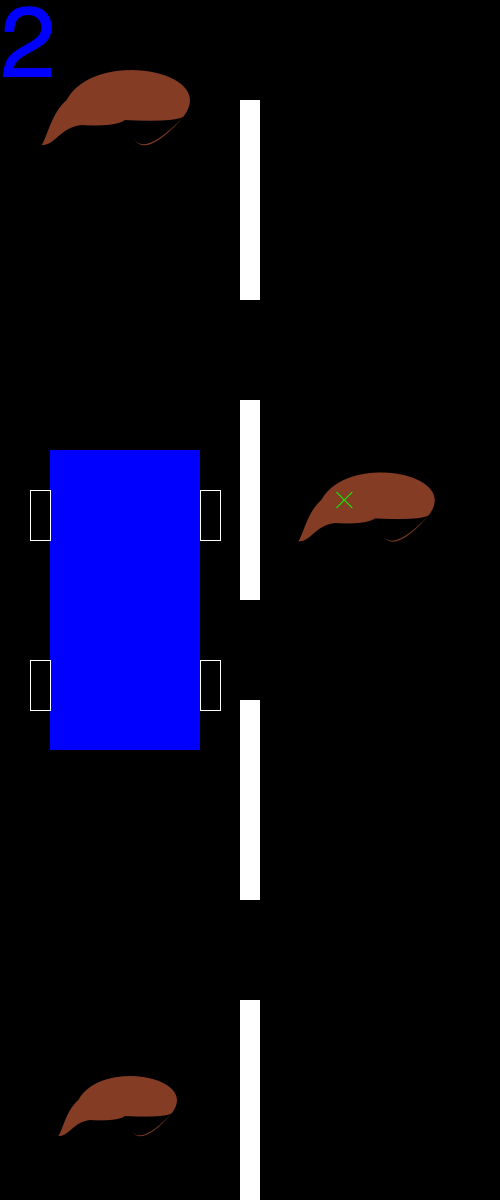
\includegraphics[height=0.4\textheight]{i1world/dillo-world}
  \caption{Gürteltiere auf der Straße}
  \label{fig:dillo-world}
\end{figure}

Ein Gürteltier allein macht noch kein Videospiel: Wir setzen gleich
mehrere Gürteltiere auf die Straße und~-- natürlich~-- überfahren sie
dann.  Das sieht dann so aus wie in
Abbildung~\ref{fig:dillo-world}. Das Auto bewegt sich auf der Straße
und kann entweder auf die linke oder rechte Straßenseite wechseln, wo
es dann gegebenfalls über Gürteltiere fährt.  Oben links steht ein
Punktestand~-- wieviele Gürteltiere schon vom lebenden Zustand in den
toten überführt wurden.

Damit wir das alles darstellen können, müssen wir ein Modell bauen,
in dem alle Informationen festgehalten sind, die auf dem Bild der
Straße zu sehen sind:
%
\begin{itemize}
\item die Position des Autos
\item die Positionen der Gürteltiere zusammen mit ihren Zuständen
\item der Punktestand
\end{itemize}
%
Wir müssen auch berücksichtigen, dass die Zeit vergeht.  Das Auto
fährt mit konstanter Geschwindigkeit, seine Position hängt also von
der Zeit ab.  Wenn wir die Zeit haben, können wir die Position des
Autos entlang der Straße daraus berechnen, wir müssen nur noch wissen,
ob das Auto links oder rechts fährt.

Man sieht schon, dass "<Positionen"> eine wichtige Rolle spielen,
sowohl für das Auto als auch für die Gürteltiere.  Um die
Datendefinition für das Modell zu schreiben, brauchen wir zunächst
eine für Positionen.  In dem Bild kann man sehen, dass dazu gehört,
auf welcher Seite der Straße sich etwas aufhält und bei welchem
"<Straßenmeter">.  Dabei kommt folgende beiden Datendefinitionen für
die Straßenseite und eine Position heraus:
%
\begin{lstlisting}
; Straßenseite
(define side
  (signature (enum "left" "right")))

; Eine Position auf der Straße besteht aus:
; - Straßenmeter (Abstand vom Straßenanfang in Meter)
; - Seite
(define-record position
  make-position
  position?
  (position-m-from-start real)
  (position-side side))
\end{lstlisting}
%
Als nächstes müssen wir die Idee "<Positionen der Gürteltiere zusammen
mit ihren Zuständen"> in eine Datendefinition umwandeln.  Wir machen
das erstmal für ein einzelnes Gürteltier und nennen das Konzept
"<Gürteltier auf der Straße">:
%
\begin{lstlisting}
; Ein Gürteltier auf der Straße hat folgende Eigenschaften:
; - Gürteltier-Zustand
; - Position auf der Straße
(define-record dillo-on-road
  make-dillo-on-road
  dillo-on-road?
  (dillo-on-road-state dillo)
  (dillo-on-road-position position))
\end{lstlisting}
%
Damit können wir jetzt das Modell für die Welt des Spiels
fertigstellen:
%
\begin{lstlisting}
; Die Welt des Spiels besteht aus:
; - Ticks seit Spielanfang
; - Seite, auf der das Auto fährt
; - Tiere auf der Straße
; - Punktzahl
(define-record world
  make-world
  world?
  (world-ticks natural)
  (world-car-side side)
  (world-dillos-on-road (list-of dillo-on-road))
  (world-score natural))
\end{lstlisting}
%
Das Wort "<Tick"> kommt aus dem Teachpack \texttt{universe.rkt}, wo es
28 Ticks pro Sekunde gibt.  Wir werden noch dazu kommen, wo die Ticks
genau herkommen.

\section{Straßenansichten}

Jetzt wo wir die Welt modelliert haben können wir sie auch auf den
Bildschirm bringen.  Wir fangen erstmal mit den einfachen und
offensichtlichen Elementen an: der Straße Straße, inklusive der
Markierung auf dem Mittelstreifen und deme Auto.  Die Gürteltiere
haben wir ja schon.

Damit wir einigermaßen realistisch über die Proportionen von allem
nachdenken können, messen wir alles in Metern ab und wandeln zwischen
Metern und Pixeln hin und her.  Auf unserem Bildschirm sieht ein
Verhältnis von 1m:100 Pixel gut aus.  Diese Funktionen konvertieren
hin und her:

\begin{lstlisting}
; Meter in Pixel umwandeln
(: meters->pixels (real -> real))

(define meters->pixels
  (lambda (meters)
    (* meters 100)))

; Pixel in Meter umwandeln
(: pixels->meters (real -> real))

(define pixels->meters
  (lambda (pixels)
    (/ pixels 100)))
\end{lstlisting}
%
Die Straße selbst ist nur ein schwarzes Rechteck, das ist einfach.
Schwieriger sind die Straßenmarkierungen, also abwechselnd ein weißer
und ein schwarzer Streifen.  Damit das realistisch aussieht,
definieeren wir erst einmal die Länge der Markierungen und die der Lücken:
%
\begin{lstlisting}
(define marking-height 2) ; Höhe der Streifen
(define gap-height 1) ; Höhe der Lücken
\end{lstlisting}
%
Die Markierungen und die Lücken müssen wir abwechseln
aneinanderkleben.  Wie oft fragst Du?  Nun, der texanische Highway ist
unendlich lang, das wäre schwierig.  Aber wir zeigen ja nur einen
Ausschnitt, und darum machen wir nur soviele Streifen, wie in den
Ausschnitt passen.  Wieviele das sind, hängt von der Höhe des
Ausschnitts ab.  Wir könnten natürlich von Hand nachzählen, das würde
aber bedeuten, dass wir uns frühzeitig auf die Höhe des Ausschnitts
festlegen müssten.  Um das zu vermeiden, schreiben wir erst einmal
eine Funktion, die als Eingabe die Anzahl der Streifen akzeptiert.
Wir folgen der Schablone für Funktionen auf natürlichen Zahlen:
%
\begin{lstlisting}
; Straßenmarkierung mit bestimmter Anzahl von Streifen malen
(: markings (natural -> image))

(define markings
  (lambda (n)
    (cond
      ((zero? n) empty-image)
      ((positive? n)
       (above (rectangle (meters->pixels .20)
                         (meters->pixels marking-height)
                         "solid"
                         "white")
              (rectangle (meters->pixels .20)
                         (meters->pixels gap-height)
                         "solid"
                         "black")
              (markings (- n 1)))))))
\end{lstlisting}
%
Hier jetzt die tatsächliche Höhe des Straßenabschnitts:
%
\begin{lstlisting}
(define road-window-height 12) ; Höhe des Straßenausschnitts
\end{lstlisting}
%
Die Idee, dass Du später nur diese eine Definition ändern musst, falls
Dir die Ausschnittshöhe nicht passt,, und sich dann alles andere
automatisch anpasst.

Um die Anzahl der nötigen Markierungen zu berechnen, teilen wir die
Höhe des Straßenausschnitts durch die Länge einer Markierung plus
Lücke.  Zur Sicherheit addieren noch eins drauf: Die Division könnte
nicht ganz aufgehen.  Außerdem wird möglicherweise am Ende nur ein
Teil eines Streifens zu sehen sein, auch dafür ist es gut gut, wenn im
Zweifelsfall einer mehr da ist.  Aus der Zahl machen wir schließlich
das Bild der Streifen:
%
\begin{lstlisting}
; Anzahl der nötigen Markierungen
(define marking-count
  (+ 1
     (quotient road-window-height
               (+ marking-height gap-height))))

; sichtbare Markierungen
(define visible-markings
  (markings marking-count))
\end{lstlisting}
%
Zur Erinnerung: Die Funktion \lstinline{quotient} haben wir auf
Seite~\pageref{func:quotient} eingeführt, sie teilt ganzzahlig.

Nun können wir das Bild des Straßenausschnitts zusammensetzen.  Wir
brauchen neben der Höhe auch noch die Breite und machen erstmal eine
leere Szene nur aus schwarzem Asphalt:
%
\begin{lstlisting}
; in Meter
(define road-width 5)

(define blank-road-window
  (empty-scene (meters->pixels road-width)
               (meters->pixels road-window-height)
               "black"))
\end{lstlisting}
%
Wie Mittelstreifen auf dem Straßenausschnitt platziert werden, hängt
vom Zeitpunkt ab.  Wir schreiben also eine Funktion, welche die Ticks
als Eingabe nimmt und ein Bild des Straßenausschnitts liefert:
%
\begin{lstlisting}
; Straßenausschnitt zu Zeitpunkt anzeigen
(: road-window (natural -> image))
\end{lstlisting}
%
Wir benutzen \lstinline{place-image/align} (siehe
Seite~\pageref{func:place-image-align}), um die Mittelstreifen auf den
Asphalt zu setzen:

%
\begin{lstlisting}
(define road-window
  (lambda (ticks)
    (place-image/align visible-markings
                       ...
                       ...
                       ... ...
                       blank-road-window)))
\end{lstlisting}
%
Wir setzen zunächst den Bezugspunkt beim Mittelstreifen nach oben in
die Mitte:
%
\begin{lstlisting}
(define road-window
  (lambda (ticks)
    (place-image/align visible-markings
                       ...
                       ...
                       "center" "top"
                       blank-road-window)))
\end{lstlisting}
%
In X-Richtung muss der Mittelstreifen in die Mitte, da können wir
einfach die Breite der Straße halbieren.

Bei der Y-Koordinate ist es schwieriger: Die hängt davon ab, wieweit
wir schon gefahren sind, und das hängt von den Ticks ab.  Wir rechnen
zunächst die Ticks in Meter um:
%
\begin{lstlisting}
(meters->pixels (ticks->meters ticks))
\end{lstlisting}
%
Das ist natürlich mehr als der Ausschnitt hoch beziehungsweise das
Mittelstreifenbild lang ist.  Das Mittelstreifenbild wiederholt sich
aber immer, wenn ein Streifen plus Lücke vorbeigezogen ist.  Wir
rechnen also die Anzahl der Pixel dafür aus:
%
\begin{lstlisting}
(define marking-segment-pixels
  (meters->pixels (+ marking-height gap-height)))
\end{lstlisting}
%
Durch diese Zahl teilen wir und nehmen den Divisionsrest, um die
Y-Position zu bekommen.  Das heißt nicht ganz~-- der Divisionsrest ist immer
positiv, und damit ist der Mittelstreifen zu weit unten: Wir ziehen
das Bild noch um einen Streifen nach oben, indem wir
\lstinline{marking-segment-pixels} abziehen.  Das kommt dabei heraus:
%
\begin{lstlisting}
(define road-window
  (lambda (ticks)
    (place-image/align visible-markings
                       (/ (image-width blank-road-window) 2)
                       (- (remainder (meters->pixels
                                       (ticks->meters ticks))
                                     marking-segment-pixels)
                        marking-segment-pixels)
                       "center" "top"
                       blank-road-window)))

\end{lstlisting}
%
\begin{aufgabeinline}
  Probiere \lstinline{road-window} aus.  Entferne die Substraktion von
  \lstinline{marking-segment-pixels} und untersucht, wie sich das
  auswirkt!
\end{aufgabeinline}
%
Die Straße ist fertig, als nächstes ist das Auto dran.  Wir fangen mit
einem Rad an:
%
\begin{lstlisting}
; Rad
(define wheel
  (rectangle (meters->pixels 0.2) (meters->pixels .5) "outline" "white"))
\end{lstlisting}
%
Als nächstes setzen wir zwei Räder zu einem Bild zusammen, das dann
links und rechts von der Karosserie platziert werden:
%
\begin{lstlisting}
; Zwei Räder auf einer Seite des Autos
(define wheels-on-one-side
 (above wheel (rectangle 0 (meters->pixels 1.2) "solid" "black") wheel))

; Bild des Autos
(define car
  (beside
   wheels-on-one-side
   (rectangle (meters->pixels car-width) (meters->pixels car-length) "solid" "blue")
   wheels-on-one-side))
\end{lstlisting}
%
Schließlich müssen wir Auto und auch die Gürteltiere noch auf der
Straße platzieren.  Wir müssen erstmal überlegen, welche Signatur die
Funktion überhaupt hat.  Klar ist, dass ein Bild herauskommen soll.
Als Eingaben stehen schon einmal fest:
%
\begin{itemize}
\item das Bild, das auf der Straße platziert werden soll
\item die Position des Bildes
\end{itemize}
%
Wir benötigen außerdem noch:
%
\begin{itemize}
\item die Zeit, weil sie bestimmt, welcher Ausschnitt der Straße
  angezeigt wird
\item das Bild der Straße
\end{itemize}
%
Letzteres überrascht Dich vielleicht. Ist das Bild der Straße nicht
immer das gleiche?  Nein, ist es nicht!  Zunächst einmal ist die
Position des Mittelstreifens je nach Zeit immer unterschiedlich.
Außerdem wollen wir ja nicht nur ein Objekt auf der Straße platzieren,
sondern viele.  Dafür füttern wir das Ergebnis der Funktion wieder in
die Funktion hinein, um ein weiteres Objekt zu platzieren.

Kurzbeschreibung, Signatur und Gerüst sehen entsprechend aus wie
folgt:
%
\begin{lstlisting}
; Bild auf der Straße platzieren
(: place-image-on-road (image natural image position -> image))

(define place-image-on-road
  (lambda (road-image ticks image position)
    ...))
\end{lstlisting}
%
\begin{figure}[tb]
  \centering
  \def\svgwidth{0.4\textwidth}
  \input{i1world/dillo-on-road.pdf_tex}
  \caption{Bild auf Straße platzieren}
  \label{fig:dillo-on-road}
\end{figure}
%
Wir müssen jetzt die Pixelkoordinaten des Bildes relativ zum
Straßenausschnitt berechnen.  Sowas plant man am besten anhand einer
Zeichnung wie der in Abbildung~\ref{fig:dillo-on-road}.
Dort sind einige Zwischengrößen eingezeichnet, die sinnvollerweise
eigene Namen bekommen:
%
\begin{description}
\item[\lstinline{road-top-m}] die Straßenmeter des oberen Randes des
  Straßenausschnitts
\item[\lstinline{road-bottom-m}] die Straßenmeter des unteren Randes des
  Straßenausschnitts
\item[\lstinline{image-m-from-start}] die Straßenmeter des
  Mittelpunkts des Bilds
\item[\lstinline{image-height-m}] die Höhe des Bildes in Meter
\end{description}
%
Die Größe \lstinline{road-top-m} wählen wir so, dass sie am Anfang des
Spiels~-- also wenn \lstinline{ticks} 0 ist~-- genau in der Mitte der
Straße ist:
%
\begin{lstlisting}
(define place-image-on-road
  (lambda (road-image ticks image position)
    ; Straßenmeter des oberen Randes des Straßenausschnitts
    (define road-bottom-m (- (ticks->meters ticks)
                             ; damit 0 in der Mitte der Ansicht ist
                             (/ road-window-height 2)))
    ; Straßenmeter des unteren Randes des Straßenausschnitts
    (define road-top-m (+ road-bottom-m road-window-height))
    ; Straßenmeter des Mittelpunkts des Bilds
    (define image-m-from-start (position-m-from-start position))
    ; Höhe des Bilds
    (define image-height-m (pixels->meters (image-height image)))
    ...))
\end{lstlisting}
%
Als nächstes rechnen wir die X-Koordinate des Bildes aus.  Dazu nehmen
wir die Mitte des Bildes zur Hand, da wo der Mittelstreifen ist.
Links ist gerade bei der Hälfte davon, rechts entsprechend:
%
\begin{lstlisting}
    (define side (position-side position))
    ; X-Koordinate der Mitte der Straße, in Pixeln
    (define middle-pixels (/ (image-width road-image) 2))
    ; X-Koordinate des Mittelpunkts des Bilds
    (define pixels-from-left
      (cond
        ((string=? side "left")
         (* middle-pixels 0.5)) ; Mitte der linken Spur
        ((string=? side "right")
         (* middle-pixels 1.5)))) ; Mitte der rechten Spur
\end{lstlisting}
%
Jetzt müssen wir nur noch überprüfen, ob das Bild überhaupt in diesem
Straßenausschnitt zu sehen   Dabei spielt
\lstinline{image-m-height} eine Rolle.    Bei der Platzierung des
Bildes müssen wir außerdem noch berücksichtigen, dass in unserem Spiel
die Y-Koordinaten von unten nach oben laufen, im Teachpack aber in die
andere Richtung.  Hier ist die fertige Funktion:
%
\begin{lstlisting}
(define place-image-on-road
  (lambda (road-image ticks image position)
    ; Straßenmeter des oberen Randes des Straßenausschnitts
    (define road-bottom-m (- (ticks->meters ticks)
                             ; damit 0 in der Mitte der Ansicht ist
                             (/ road-window-height 2)))
    ; Straßenmeter des unteren Randes des Straßenausschnitts
    (define road-top-m (+ road-bottom-m road-window-height))
    ; Straßenmeter des Mittelpunkts des Bilds
    (define image-m-from-start (position-m-from-start position))
    ; Höhe des Bilds
    (define image-height-m (pixels->meters (image-height image)))

    (define side (position-side position))
    ; X-Koordinate der Mitte der Straße, in Pixeln
    (define middle-pixels (/ (image-width road-image) 2))
    ; X-Koordinate des Mittelpunkts des Bilds
    (define pixels-from-left
      (cond
        ((string=? side "left")
         (* middle-pixels 0.5)) ; Mitte der linken Spur
        ((string=? side "right")
         (* middle-pixels 1.5)))) ; Mitte der rechten Spur
    (if (and (>= (+ image-m-from-start (/ image-height-m 2))
                 road-bottom-m)
             (<= (- image-m-from-start (/ image-height-m 2))
                 road-top-m))
        (place-image/align
         image
         pixels-from-left
         (- (image-height road-image)
            (meters->pixels (- image-m-from-start road-bottom-m)))
         "center" "center"
         road-image)
        road-image)))
\end{lstlisting}
%
FIXME
% 
\begin{lstlisting}
; Auto auf die Straße setzen
(: place-car-on-road (natural position image -> image))
                      
(define place-car-on-road
  (lambda (ticks car-position road-image)
    (place-image-on-road road-image
                         ticks
                         car car-position)))


; Ein Tier auf die Straße malen
(: place-dillo-on-road (natural dillo-on-road image -> image))

(define place-dillo-on-road
  (lambda (ticks dillo-on-road road-image)
    (place-image-on-road road-image
                         ticks
                         (dillo-image (dillo-on-road-state dillo-on-road))
                         (dillo-on-road-position dillo-on-road))))
\end{lstlisting}
%
\begin{lstlisting}
; Alle Tiere auf die Straße malen
(: place-dillos-on-road (natural (list-of dillo-on-road) image -> image))

(define place-dillos-on-road
  (lambda (ticks dillos-on-road road-image)
    (fold road-image
          (lambda (dillo-on-road image)
            (place-dillo-on-road ticks dillo-on-road image))
          dillos-on-road)))
\end{lstlisting}

\begin{lstlisting}
; Punktzahl anzeigen
(: place-score (natural image -> image))

(define place-score
  (lambda (score image)
    (place-image/align
     (text (number->string score) 100 "blue")
     0 0
     "left" "top"
     image)))

; Spiel anzeigen
(: world->image (world -> image))

(define world->image
  (lambda (world)
    (define ticks (world-ticks world))
    (place-score
     (world-score world)
     (place-car-on-road
      ticks
      (world-car-position world)
      (place-dillos-on-road
       ticks
       (world-dillos-on-road world)
       (road-window ticks))))))
\end{lstlisting}

FIXME: verschiedene Beispiele zum Ausprobieren animieren

\section{Welt in Bewegung}
  
Wie kommen wir von hier zu einem fertigen Spiel?  Wir denken darüber
nach, was wir alles noch brauchen werden, damit aus dem
\lstinline{world}-Record alle Aspekte des Spiels berechnet werden
können, mithin der texanische Highway simuliert:\label{page:dillo-world-todos}
%
\begin{enumerate}
\item Wir brauchen für die Darstellung die Position des Autos~-- als
  \lstinline{position}-Record, nicht bloß die Straßenseite.
\item Wir müssen feststellen ob das Auto die Position eines
  Gürteltiers berührt und dieses damit überfährt.
\item Wir müssen zählen, wieviele Tiere vo einem gegebenen
  Zeitpunkt vom Auto touchiert, mithin überfahren werden, damit wir
  die Punktzahl entsprechend erhöhen können.
\item Schließlich müssen wir alle Tiere überfahren, deren Position
  unter das Auto gerät.
\end{enumerate}
%
Diese Liste arbeiten wir jetzt ab.
%
\paragraph{Position des Autors}
Fangen wir an mit der Position des Autos: Die Seite steht ja schon im
\lstinline{world}-Record.  Für die Konstruktion einer Position fehlen
noch die Straßenmeter, die aus den Ticks berechnet werden können.  Die
Funktion dafür hat Kurzbeschreibung, Signatur und Testfälle wie folgt:
%
\begin{lstlisting}
; Position des Autos
(: world-car-position (world -> position))
\end{lstlisting}
%
Für die Testfälle und auch für die Konstruktion der Funktion müssen
wir von Ticks in Straßenmeter umrechnen.  Diese Umrechnung ist eine
Zwischengröße bei der Berechnung der Position, wir verlagern sie
deswegen in eine separate Funktion namens \lstinline{ticks->meters}.
Wir haben sie geschrieben, bevor wir mit
\lstinline{world-car-position} weitergemacht haben.  Du kannst aber
auch genauso gut erstmal \lstinline{world-car-position}
fertigschreiben und erst dann \lstinline{ticks->meters} entwickeln.
Wir müssen zunächst einmal festlegen, wie schnell der Wagen fährt.
Wir haben uns für ein recht gemächliches Tempo entschieden, damit auch
wirklich alle Gürteltiere erwischen:
%
\begin{lstlisting}
; Meter pro Tick
(define meters-per-tick 0.1)
\end{lstlisting}
%
Diese Funktion ist so einfach, dass sich ausnahmsweise separates
Testen nicht lohnt:
%
\begin{lstlisting}
; Ticks in Meter umwandeln
(: ticks->meters (natural -> rational))

(define ticks->meters
  (lambda (ticks)
    (* meters-per-tick ticks)))
\end{lstlisting}
%
Weiter geht es mit den Tests von \lstinline{world-car-position}, bei
denen wir \lstinline{ticks->meters} benutzen können:
%
\begin{lstlisting}
(check-expect (world-car-position (make-world 0 "left" empty 0))
              (make-position 0 "left"))
(check-expect (world-car-position (make-world 100 "right" empty 0))
              (make-position (ticks->meters 100) "right"))
\end{lstlisting}
%
Die Schablone für die Funktion berücksichtigt, dass es sich sowohl bei
Ein- als auch bei der Ausgabe jeweils um zusammengesetzte Daten handelt:
%
\begin{lstlisting}
(define world-car-position
  (lambda (world)
    (make-position ... ...)
    ...
    (world-ticks world)
    (world-car-side world)
    (world-dillos-on-road world)
    (world-score world)
    ...))
\end{lstlisting}
%
Nur die ersten beiden Felder von \lstinline{world} sind relevant für
die Position des Autos~-- Gürteltiere und Punktzahl sind sichtlich
nicht relevant.  Für die Position brauchen wir die Straßenmeter, die
wir aus den Ticks mit Hilfe von \lstinline{ticks->meters} berechnen
können:
%
\begin{lstlisting}
(define world-car-position
  (lambda (world)
    (make-position (ticks->meters (world-ticks world))
                   (world-car-side world))))
\end{lstlisting}
%
\paragraph{Berührung eines Gürteltiers} Als nächstes auf der Liste auf
Seite~\pageref{page:dillo-world-todos} müssen wir feststellen, ob das
Auto die Position eines Gürteltiers berührt.  Dafür ist natürlich
relevant, wie groß das Auto ist.  Wir haben uns für folgende Maße
entschieden:
%
\begin{lstlisting}
; Breite des Autos
(define car-width 1.5)
; Länge des Autos
(define car-length 3.0)
\end{lstlisting}
%
Wir brauchen eine Funktion mit Kurzbeschreibung und Signatur wie
folgt:
%
\begin{lstlisting}
; Berührt das Auto eine Position?
(: car-on-position? (position position -> boolean))
\end{lstlisting}
%
Das Auto berührt eine Position, wenn die Position auf der gleichen
Straßenseite nah dran ist.  Hier die Testfälle dazu:
%
\begin{lstlisting}
(check-expect (car-on-position? (make-position 10 "left")
                                (make-position 10 "right"))
              #f)
(check-expect (car-on-position? (make-position 10 "left")
                                (make-position 10 "left"))
              #t)
(check-expect (car-on-position? (make-position 11 "left")
                                (make-position 10 "left"))
              #t)
(check-expect (car-on-position? (make-position 10 "left")
                                (make-position 11 "left"))
              #t)
\end{lstlisting}
%
Für die Schablone haben wir es bei beiden Eingaben mit
zusammengesetzten Daten zu tun:
%
\begin{lstlisting}
(define car-on-position?
  (lambda (car-position position)
    ...
    (position-side car-position) 
    (position-side position)
    (position-m-from-start car-position)
    (position-m-from-start position)
    ...))
\end{lstlisting}
%
Die beiden Straßenseiten müssen gleich sein.  Bei den Straßenmetern
der beiden Positionen ist relevant, dass die Straßenmeter des Autos
genau in der Mitte des Autos sind~-- die Position darf nicht mehr als
die Hälfte davon entfernt sein.  Um den Vergleich zu erleichtern, egal
ob die Position vor oder hinter dem Mittelpunkt ist, benutzen wir die
eingebaute Funktion \lstinline{abs}\index{abs@\texttt{abs}}.  Diese
Funktion berechnet den \textit{Absolutbetrag}\index{Absolutbetrag}
einer Zahl: Sie macht aus negativen Zahlen die entsprechenden
positiven Zahlen:
%
\begin{lstlisting}
(abs 5)
|\evalsto| 5
(abs -5)
|\evalsto| 5
\end{lstlisting}
%
Hier die fertige Funktion:
%
\begin{lstlisting}
(define car-on-position?
  (lambda (car-position position)
    (and (string=? (position-side car-position) 
                   (position-side position))
         (<= (abs (- (position-m-from-start car-position)
                     (position-m-from-start position)))
             (/ car-length 2)))))
\end{lstlisting}

\paragraph{Wieviele Tiere sind gerade unter dem Auto?} Als nächstes
schreiben wir eine Funtkion, welche die Tiere unter dem Auto zählt,
damit wir die Punktzahl entsprechend erhöhen können.  Genauer gesagt
zählen wir nur die \emph{lebendigen} Gürteltiere: Für das nochmalige
Überfahren eines toten Gürteltiers gibt es keinen Punkt.  Hier
Kurzbeschreibung und Signatur:
%
\begin{lstlisting}
; Wieviele Tiere werden vom Auto berührt?
(: live-dillos-under-car-count 
   (position (list-of dillo-on-road) -> natural))
\end{lstlisting}
%
Für den Test sollten wir in der Eingabe sowohl lebendige als auch
tote Gürteltiere unterbringen, ebenso wie solche, die unter dem Auto
liegen, und solche, die weiter weg sind:
%
\begin{lstlisting}
(check-expect
  (live-dillos-under-car-count
    (make-position 10 "left")
     (list (make-dillo-on-road dillo1 (make-position 10 "left"))
           (make-dillo-on-road dillo2 (make-position 10 "right"))
           (make-dillo-on-road dillo2 (make-position 11 "left"))
           (make-dillo-on-road dillo1 (make-position 9 "left"))
           (make-dillo-on-road dillo1 (make-position 12 "left"))))
  2)
\end{lstlisting}
%
Der Test zählt das erste und das vorletzte Gürteltier.

Für die Definition könnten wir die Schablone für Funktionen auf Listen
heranziehen.  Da es aber darum geht, aus einer Liste einige Elemente
auszuwählen, die einem bestimmten Kriterium entsprechen, können wir
auch die Funktion \lstinline{filter} von Seite~\pageref{func:filter}
benutzen, die eingebaute Version von \lstinline{extract-list}.  Damit
extrahieren wir die zu zählenden Gürteltiere.  Die müssen wir nur noch
mit der ebenfalls eingebauten Funktion~\lstinline{length}
zählen. (\lstinline{Length} ist die eingebaute Version von
\lstinline{list-length}, siehe Seite~\pageref{func:length}.)
%
\begin{lstlisting}
(define live-dillos-under-car-count
  (lambda (car-position dillos-on-road)
    (length
     (filter (lambda (dillo-on-road)
               (and (car-on-position?
                       car-position
                       (dillo-on-road-position dillo-on-road))
                    (dillo-alive? 
                      (dillo-on-road-state dillo-on-road))))
             dillos-on-road))))
\end{lstlisting}

\paragraph{Gürteltiere tatsächlich überfahren} Als letzter
Arbeitsauftrag bleibt noch, die Gürteltiere, die vom Auto touchiert
werden, vom lebenden in den toten Zustand zu überführen.  Die Funktion
akzeptiert wie \lstinline{live-dillos-under-car-count} die Position
des Autos und die Gürteltiere:
%
\begin{lstlisting}
; Alle Tiere überfahren, die das Auto berührt
(: run-over-dillos-on-road
   (position (list-of dillo-on-road) -> (list-of dillo-on-road)))
\end{lstlisting}
%
Beim Testen gibt es jede Menge tote Gürteltiere, darum definieren wir
den dazugehörigen Zustand zwecks Wiederverwendung:
%
\begin{lstlisting}
(define dead-dillo1 (run-over-dillo dillo1))

(check-expect
 (run-over-dillos-on-road
  (make-position 10 "left")
  (list (make-dillo-on-road dillo1 (make-position 10 "left"))
        (make-dillo-on-road dillo1 (make-position 10 "right"))
        (make-dillo-on-road dillo1 (make-position 11 "left"))
        (make-dillo-on-road dillo1 (make-position 9 "left"))
        (make-dillo-on-road dillo1 (make-position 12 "left"))))
 (list (make-dillo-on-road dead-dillo1 (make-position 10 "left"))
       (make-dillo-on-road dillo1 (make-position 10 "right"))
       (make-dillo-on-road dead-dillo1 (make-position 11 "left"))
       (make-dillo-on-road dead-dillo1 (make-position 9 "left"))
       (make-dillo-on-road dillo1 (make-position 12 "left"))))
\end{lstlisting}
%
Die Funktion wendet also eine Operation auf jedes Element der Liste an
und gibt uns die Ergebnisse in einer Liste zurück: Dafür können wir
wieder eine Higher"=Order"=Funktion aus Kapitel~\ref{cha:higher-order}
verwenden, nämlich \lstinline{map}, die eingebaute Version von
\lstinline{list-map}, siehe Seite~\pageref{func:map}.  Für jedes
Gürteltier überprüft die Funktion, ob es vom Auto berührt wird und
benutzt gegebenenfalls \lstinline{run-over-dillo}, um die schmutzige
Arbeit zu machen:

FIXME: KA
%
\begin{lstlisting}
(define run-over-dillos-on-road
  (lambda (car-position dillos-on-road)
    (map (lambda (dillo-on-road)
           (if (car-on-position?
                car-position
                (dillo-on-road-position dillo-on-road))
               (make-dillo-on-road
                (run-over-dillo (dillo-on-road-state dillo-on-road))
                (dillo-on-road-position dillo-on-road))
               dillo-on-road))
         dillos-on-road)))
\end{lstlisting}

\begin{aufgabeinline}
  Was ist die Konsequenz, wenn auch das Überfahren toter Gürteltiere
  Punkte geben würde?  Versuche, das hier schon einmal durch reines
  Nachdenken zu klären und probiere es später aus!

  FIXME: nochmal aufgreifen
\end{aufgabeinline}

\section{Bewegung und Zustand}

TBD  Dafür ist ein weiteres Teachpack namens
\texttt{universe.ss}\index{universe.ss@\texttt{universe.ss}} zuständig.  Es
kann in \drscheme{} genauso wie bei \texttt{image.rkt}
geladen werden.  

Alle Definitionen von
\texttt{image.rkt} sind auch in \texttt{universe.ss} verfügbar.

In der Terminologie von \texttt{universe.ss} ist ein Modell eine
\textit{world}, auf deutsch eine \textit{Welt}: Die Idee dahinter
ist, dass ein Bild eine Ansicht einer kleinen Welt ist.  Damit das
funktioniert, muss bei \texttt{universe.ss} eine erste Welt angemeldet
werden, zusammen mit Angaben, wie groß die Ansicht wird.  Dazu gibt es
die Funktion \texttt{big-bang}\index{big-bang@\texttt{big-bang}}:
%
\begin{lstlisting}
(: big-bang (natural natural number world -> #t))
\end{lstlisting}
%
("<Big Bang"> heißt zu deutsch "<Urknall">.)
Die ersten beiden Argumente geben Breite und Höhe der Ansicht an.  Das
dritte Argument gibt die Dauer (in Sekunden) zwischen Ticks der Uhr
an, die für die Animation benötigt wird.  Das vierte Argument gibt
schließlich die erste Welt an.  (Der Rückgabewert, immer
\lstinline{#t}, ist ohne Bedeutung.)  Für den Himmel mit
Sonne sieht der Aufruf von \texttt{big-bang} folgendermaßen aus:
%
\begin{lstlisting}
(big-bang sky-width sky-height 0.1 0)
\end{lstlisting}
%
Dieser Aufruf erzeugt ein Fenster mit Breite und Höhe des Himmels,
startet die Uhr, die jede Sekunde zehnmal tickt, und legt als erste
Welt "<0">, also den Anfang der Zeit fest.  (Eine zehntel Sekunde
reicht etwa aus, damit die Animation dem menschlichen Auge als
"<Bewegung"> erscheint.)

Damit das Teachpack die Welt in eine Ansicht umwandeln kann, muss eine
entsprechende Ansicht angemeldet werden.  Dafür ist die Funktion
\texttt{on-redraw\index{on-redraw@\texttt{on-redraw}}} zuständig:
%
\begin{lstlisting}
(: on-redraw ((world -> image) -> #t))
\end{lstlisting}
%
Als Argument akzeptiert \texttt{on-redraw} also eine Funktion, die aus
einer Welt ein Bild macht.  TBD

Auch diese Funktion muss noch beim Teachpack angemeldet werden.  Dafür
die Teachpack-Funktion
\texttt{on-tick-event\index{on-tick-event@\texttt{on-tick-event}}}
zuständig:
%
\begin{lstlisting}
(: on-tick-event ((world -> world) -> #t))
\end{lstlisting}
%
Die \texttt{on-tick-event}-Funktion akzeptiert eine Funktion, die bei
jedem Uhren-Tick aufgerufen wird, um aus der "<alten"> Welt eine neue
zu machen.  Auf diese Beschreibung und auch auf die Signatur
passt aber \texttt{next-time}.  Der Aufruf kann also so aussehen:
%
\begin{lstlisting}
(on-tick-event next-time)
\end{lstlisting}
%
Wenn das Programm
beendet werden soll, muss \texttt{on-tick-event} die Funktion
\texttt{end-of-time\index{end-of-time@\texttt{end-of-time}}} des
Teachpacks aufrufen, die folgende Signatur hat:
%
\begin{lstlisting}
(: end-of-time (string -> world))
\end{lstlisting}
%

\section{Andere Welten}

Eine kleine (wenn auch nicht besonders sinnvolle) Erweiterung zeigt,
wie die Animation auf Benutzereingaben reagieren kann.  Dazu muss sie
noch eine weitere Funktion anmelden, und zwar mittels
\texttt{on-key-event\index{on-key-event@\texttt{on-key-event}}}, das
ähnlich funktioniert wie \texttt{on-tick-event}:
%
\begin{lstlisting}
(: on-key-event ((world string -> world) -> #t))
\end{lstlisting}
%
Die Funktion, die mit \texttt{on-key-event} angemeldet wird, wird
immer aufgerufen, wenn der Benutzer eine Taste drückt.  Welche Taste
gedrückt wurde, gibt das zweite Argument 
an.  Wenn der Benutzer eine reguläre Zeichen-Taste drückt (also keine
Cursor-Taste o.ä.), ist dieses Argument eine Zeichenkette bestehend
aus diesem einen Zeichen.

TBD

\section*{Aufgaben}

TBD

\begin{aufgabe}
  Schreiben Sie ein kleines Telespiel Ihrer Wahl.
\end{aufgabe}

%%% Local Variables: 
%%% mode: latex
%%% TeX-master: "i1"
%%% End: 

